
% Первая глава работы 
\chapter{Теоретическое введение}
\label{chap1}

\section{Методы моделирования}
\label{chap1:sec1}

%\subsection{Аналитическое моделирование}

\emph{Натурным моделированием} называют проведение исследования на настоящем
предмете с последующей обработкой результатов опыта на основе теории
подобия. Натруное моделирование разделяется на научный эксперимент,
комплексные испытания и производственный эксперимент. Научный
эксперимент характеризуется обширным применением средств
автоматизации, использованием весьма всевозможных средств обработки
информации, возможностью вмешательства человека в процесс выполнения
эксперимента.

%\subsection{Имитационное моделирование}

\emph{Имитационное моделирование} --- это способ исследования, при котором
исследуемая система сменяется моделью, с достаточной точностью
описывающей настоящую систему, с которой проводятся опыты с целью
извлечения информации об этой системе. Такую модель можно «проиграть»
во времени, как для одного испытания, так и заданного их множества.



\section{Алгоритмы управления очередями}
\label{chap1:sec2}

Алгоритмы управления и обработки очереди разделяются на два основных класса:

Алгоритмы пассивного управления очередью (PQM) \cite{pqm} --- класс алгоритмов,
применяемых для обработки очередей, при котором при достижении порогового
значения, алгоритм отбрасывает пакеты в соответствии с некоторым правилом
конкретной реализации алгоритма. Данные алгоритмы просты в исполнении, однако
лишены возможности адаптироваться под разные нагрузки. 

Примеры алгоритмов пассивного управления очередью:

\begin{itemize}
  \item DropTail --- отбрасывает пакеты с конца очереди
  \item DropHead --- отбрасывает пакеты с начала очереди 
  \item RandomDrop --- отбрасывает случайные пакеты из очереди 
\end{itemize}

% subsection Пример (end)

В маршрутизаторах и коммутаторах активное управление очередью (AQM) \cite{aqm} относится к
процессу отбрасывания пакетов внутри буфера, связанного с контроллером сетевого
интерфейса (NIC), до того, как этот буфер заполнится, с целью уменьшения
перегрузки сети или повышения сквозной производительности.

Примеры алгоритмов активного управления очередью (а также статьи с подробным
описанием каждого из алгоритмов, так как покрыть каждый из этих алгоритмов в рамках данной работы не получится):

\begin{itemize}
    \item RED \cite{RandomEarlyDeFloyd1993, ASelfConfigurFeng1999}
    \item ARED \cite{ARED_1, ARED_2, ARED_3, AnalysisOfAdaLaR2003} 
    \item BLUE \cite{blue}
    \item GRED \cite{RevisitingTheHamadn2019}
\end{itemize}

В данной работе будут изучены лишь 3 алгоритма, в связи с тем, что они уже
используются в сетевом стеке ядра Linux, а также средстве имитационного
моделирования NS-2. А именно:

\begin{itemize}
  \item DropTail --- как базовый алгоритм пассивного управления очередью;
  \item RED --- как классический алгоритм активного управления очередью;
  \item ARED --- в качестве сравнения динамического \footnote{Под динамическим подразумевается алгоритм, который в процессе своей работы подстраивает параметры системы. Подробнее об этом в разделе \ref{chap1:sec3:sub4}} алгоритма с классическим;
\end{itemize}

\section{Алгоритмы активного управления очередью семейства RED}
\label{chap1:sec3}

\subsection{RED}
\label{chap1:sec3:sub1}

RED \cite{red-1993} (Random Early Detection, произвольное раннее
обнаружение) --- алгоритм активного управления очередью (AQM) для
управления переполнением очередей маршрутизаторов с возможность
предотвращения перегрузок.

Веpоятность $p_{b}$ маркиpовки на отбpасывание пакетов пpедставляет
собой функцию, линейно зависящую от $\hat{q}$, минимального $q_{\min}$
и максимального $q_{\max}$ пороговых значений и параметра $p_{\max}$,
определяющего часть отбрасываемых пакетов при достижении средним
размером очереди значения $q_{\max}$ и вычисляется следующим образом:

\[
p_{b} = \left\{
  \begin{aligned}
& 0, &&    0 < \hat{q} \leqslant q_{\min}, \\
& \frac{\hat{q} - q_{\min}}{q_{\max} - q_{\min}} p_{\max}, &&  q_{\min} < \hat{q} \leqslant q_{\max} ,\\
& 1, &&   \hat{q} > q_{\max}. 
  \end{aligned}
\right.
\]

\subsection{Разбор алгоритма RED}
\label{chap1:sec3:sub2}

Пакет при поступлении в систему попадает в модуль сброса. Решение о
сбросе пакета принимается на основе значения вероятности $p$,
получаемого от управляющего модуля. Вероятность $p$ сброса пакетов
зависит от экспоненциально взвешенного скользящего среднего размера
длины очереди $\hat{q}$, также вычисляемого управляющим модулем,
основываясь на текущем значении длины очереди $q$ (см. рис.~\ref{fig:red:1.1}).

\begin{figure}[H]
  \centering
  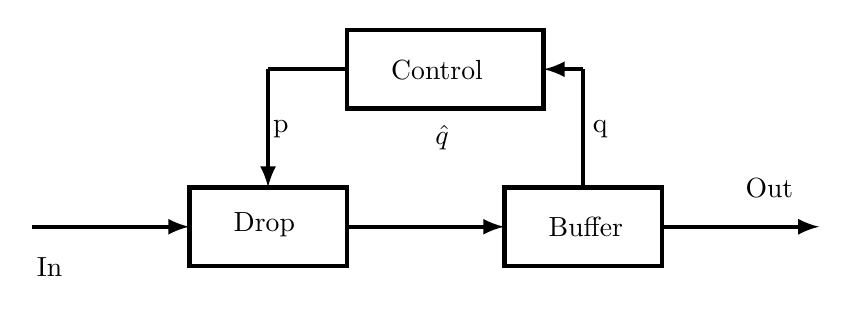
\begin{tikzpicture}
    \draw[draw=black, ultra thick, solid] (-2.00,3.00) rectangle (0.50,2.00);
    \draw[draw=black, ultra thick, solid] (-4.00,1.00) rectangle (-2.00,0.00);
    \draw[draw=black, ultra thick, solid] (0.00,1.00) rectangle (2.00,0.00);
    \draw[draw=black, -latex, ultra thick, solid] (-6.00,0.50) -- (-4.00,0.50);
    \draw[draw=black, -latex, ultra thick, solid] (-2.00,0.50) -- (0.00,0.50);
    \draw[draw=black, -latex, ultra thick, solid] (2.00,0.50) -- (4.00,0.50);
    \draw[draw=black, ultra thick, solid] (1.00,1.00) -- (1.00,2.50);
    \draw[draw=black, ultra thick, solid] (-2.00,2.50) -- (-3.00,2.50);
    \draw[draw=black, -latex, ultra thick, solid] (1.00,2.50) -- (0.50,2.50);
    \draw[draw=black, -latex, ultra thick, solid] (-3.00,2.50) -- (-3.00,1.00);
    \node[black, anchor=south west] at (-3.56,0.25) {Drop};
    \node[black, anchor=south west] at (0.44,0.25) {Buffer};
    \node[black, anchor=south west] at (-6.06,-0.25) {In};
    \node[black, anchor=south west] at (-3.06, 1.5) {p};
    \node[black, anchor=south west] at (1, 1.5) {q};
    \node[black, anchor=south west] at (-1, 1.35) {$\hat{q}$};
    \node[black, anchor=south west] at (2.94,0.75) {Out};
    \node[black, anchor=south west] at (-1.56,2.25) {Control};
  \end{tikzpicture}
  \caption{Модуль RED}
  \label{fig:red:1.1}
\end{figure}

Гpафик веpоятности потери пакета в зависимости от сpеднего размера
очереди приведен на графике ~\ref{fig:red:1.2}.
%будет выглядеть следующим образом:


\begin{figure}[H]
  \centering
  \begin{tikzpicture}
    \draw[draw=black, -latex, very thick, solid] (-4.00,-3.00) -- (5.00,-3.00);
    \draw[draw=black, -latex, very thick, solid] (-4.00,-3.00) -- (-4.00,4.00);
    \node[black, anchor=south west] at (1.44,-3.5) {$q_{\max}$};
    \node[black, anchor=south west] at (-2.56,-3.5) {$q_{\max}$};
    \node[black, anchor=south west] at (-4.5,-3.5) {0};
    \node[black, anchor=south west] at (-5.,-0.25) {$p_{\max}$};
    \draw[draw=black, ultra thick, solid] (-2.00,-3.00) -- (2.00,0.00);
    \draw[draw=black, semithick, dotted] (2.00,0.00) -- (2.00,3.00);
    \draw[draw=black, ultra thick, solid] (2.00,3.00) -- (5.00,3.00);
    \draw[draw=black, semithick, dotted] (2.00,0.00) -- (2.00,-3.00);
    \draw[draw=black, semithick, dotted] (-4.00,0.00) -- (2.00,0.00);
    \node[black, anchor=south west] at (-4.56,2.95) {1};
    \node[black, anchor=south west] at (4.94,-3.25) {q};
    \node[black, anchor=south west] at (-4.06,3.7) {p};
    \draw[draw=black, semithick, dotted] (-4.00,3.00) -- (2.00,3.00);
  \end{tikzpicture}
  \caption{Вероятность потеpи пакета в RED}
  \label{fig:red:1.2}
\end{figure}

Pеализация функции пpосчета вероятности на отбpасывание пакета в алгоpитме RЕD
выглядит следующим обpазом:

\begin{algorithm}[H]
	\caption{Функция просчета вероятности на отбрасывание} 
	\begin{algorithmic}[1]
            \If {$\hat{q} \geq q_{\max}$}
                \State $p = 1$
            \Else 
              \State $p = k * \hat{q} + b$
              \Comment{график прямой от $q_{\min}$ до $q_{\max}$}
              \State $p *= q_{\max}$
            \EndIf
	\end{algorithmic} 
\end{algorithm}

\subsection{Проблемы RED}
\label{chap1:sec3:sub3}

Одна из фундаментальных проблем с дизайном RED заключается в том, что он
зависит от размера очереди как показателя рабочей нагрузки. В то время как
наличие постоянной очереди указывает на состояние перегрузки, длина очереди
предоставляет очень мало информации о серьезности состояния перегрузки. 

Из-за зависимости алгоритма RED от размера очереди ему присуща проблема точного
определения степени перегруженности. Как следствие, RED требует
правильных параметров для правильной работы в различных
сценариях перегрузки. В то время как RED может достичь идеального рабочего
состояния, это может быть достигнуто только при наличии достаточной буферной
емкости и соотминимального порога $q_{\min}$ветствующих настроек параметров.


\subsection{ARED}
\label{chap1:sec3:sub4}

В алгоритме Adaptive RED (ARED), разработанном Фенгом
\cite{ARED_1,ARED_2} и усовершенствованная С. Флойд \cite{ARED_3},
функция сброса модифицируется посредством изменения по принципу AIMD
(принцип AIMD заключается в том, что увеличение некоторой величины
производится путём сложения с некоторым параметром, у уменьшение ---
путём умножения на параметр).

Алгоритм ARED функционирует следующим образом. Для каждого интервала
interval (параметр) в секундах, если $\hat{q}$ больше целевого
(желаемого) значения $\hat{q_t}$ и $p_{\max} \leqslant 0,5$, то $p_{\max}$
увеличивается на некоторую величину $\alpha$; в противном случае, если
$\hat{q}$ меньше целевого значения $\hat{q_t}$ и $p_{\max}\geqslant 0,01$, то
$p_{\max}$ уменьшается в $\beta$ раз:

\[
p_{\max} = \left\{
  \begin{aligned}
   & p_{\max}+\alpha, && \hat{q}>\hat{q_{t}}, && p_{\max} \leqslant 0,5, \\
   & \beta * p_{\max}, && \hat{q}<\hat{q_{t}}, && p_{\max} \geqslant 0,01, 
  \end{aligned}
\right.
\]

где

\[
q_{\min}+0,4\left(q_{\max}-q_{\min}\right) < \hat{q_t} < q_{\min}+0,6\left(q_{\max}-q_{\min}\right).
\]

У алгоритма ARED есть следующие преимущества, по сравнению с классическим RED:

\begin{itemize}

  \item автоматическая установка $\hat{q_t}$ на основе пропускной способности
    соединения

  \item медленное адаптирование $p_{\max}$, для того, чтобы средний размер
    очереди находился в пределах $q_{\min}$ и $q_{\max}$, а также сама
    вероятность находилась в промежутке [0.01, 0.5] (что эквивалентно [1\%,
    50\%])

\end{itemize}

Данные изменения существенно помогают решить основную проблмеу классического
RED (которые описаны в \ref{chap1:sec3:sub3}).


\section{Средства моделирования}
\label{chap1:sec3}

\subsection{Средство имитационного моделирования ns-2}
\label{chap1:sec3:sub1}

NS-2 (Network Simulator 2) --- это симулятор дискретных событий,
предназначенный для исследования компьютерных сетей. NS-2 предоставляет
существенную поддержку для моделирования протоколов TCP, маршрутизации и
многоадресной рассылки по проводным и беспроводным (локальным и спутниковым)
сетям.

\subsection{Средство натурного моделирования Mininet}
\label{chap1:sec3:sub2}

Mininet --- это симулятор сетевых топологий, который позволяет моделировать и
анализировать поведение сети в имитируемой среде. Симулятор основан на
виртуальных машинах Linux и технологиях пространства имен, которые используются
для создания изолированных сетевых компонентов. Используя Mininet, можно
изучать различные сетевые протоколы, алгоритмы маршрутизации и методы
управления трафиком. Возможности моделирования Mininet включают создание
виртуальных сетевых узлов, настройку топологий (включая связь между узлами и
конфигурацию IP-адресов), моделирование различных сетевых условий (таких как
задержки, потеря пакетов и пропускная способность) и интеграцию с контроллерами
для изучения новых протоколов и алгоритмов.

\section{Дополнительные инструменты} % (fold)
\label{chap1:sec4}

\subsection{TC --- Traffic Control}
\label{chap1:sec4:sub1}

Linux предлагает инструменты для управления передачей пакетов и манипулирования
ими. Подсистема Linux Traffic Control (TC) помогает контролировать,
классифицировать, формировать и планировать сетевой трафик. TC также изменяет
содержимое пакетов во время классификации с помощью фильтров и действий.
Подсистема TC достигла этого за счет использования дисциплин массового
обслуживания (qdisc), фундаментальных элементов архитектуры TC. 

Механизм планирования упорядочивает ячейки перед тем, как они войдут в разные
очереди или выйдут из них. Наиболее распространенным планировщиком является
планировщик First-In-First-Out (FIFO). Можно выполнять операции с qdiscs
временно с помощью утилиты tc или постоянно с помощью NetworkManager.

\subsection{Iperf3 --- генератор TCP, UDP и SCTP трафика}
\label{chap1:sec4:sub2}

Iperf - это инструмент, используемый для активного измерения максимально
достижимой пропускной способности IP-сетей. Он позволяет пользователям
настраивать различные параметры, связанные с синхронизацией, протоколами и
размерами буфера. 

При каждом тестировании создается отчет, содержащий информацию об измеренной
пропускной способности, скорости передачи данных, потере пакетов и других
соответствующих параметрах. Программа разделена на клиентскую и серверную
части, поэтому для ее работы понадобится как минимум 2 устройства,
подключенных к сети. 

% section  (end)

%%% Local Variables:
%%% mode: latex
%%% coding: utf-8-unix
%%% TeX-master: "../default"
%%% End:
